\documentclass{article}

\usepackage{header}

\usepackage[left=2cm,right=2cm, top=2cm,bottom=2cm,bindingoffset=0cm]{geometry}

\usepackage{graphicx}
\graphicspath{.}

\usepackage{hyperref}  % so the reference URLs and citations are clickable
\usepackage{csquotes}  % needed for biblatex for babel
\usepackage[backend=biber]{biblatex}
\addbibresource{bibliography.bib}

\usepackage{titlepage}

\setUDK{004.9}
\setToResearch

\setTitle{Обратимые фильтры Блума и сравнение геномов}

% Выбрать одно из трех:
% КТ1 -- \setStageOne
% КТ2 -- \setStageTwo
% Финальная версия -- \setStageFinal
\setStageOne
%\setStageTwo
%\setStageFinal

\setGroup{206}
%сюда можно воткнуть картинку подписи
% \setStudentSgn{\smash{\includegraphics[scale=0.25]{my-sig.png}}}
\setStudentSgn{\includegraphics[scale=0.10]{my-sig.jpg}}
% \setStudentSgn{\smash{kjdfl}}
\setStudent{М.М. Марченко}
\setStudentDate{19.05.2022}
\setAdvisor{Григорий Аронович Кучеров}
\setAdvisorTitle{Ведущий научный сотрудник} %(научно-учебная лаборатория методов анализа больших данных)}
\setAdvisorAffiliation{CNRS, France}
\setAdvisorDate{}
\setGrade{}
%сюда можно воткнуть картинку подписи
\setAdvisorSgn{}
\setYear{2022}

\begin{document}

% Эта команда создает титульную страницу
\makeTitlePage

\begin{abstract}
    Invertible Bloom Lookup Table is a probabilistic data structure for storing
    key-value pairs. Notably it allows to pack and restore two 
    similar objects using O(difference) space. In this work we experiment with 
    this feature and try to apply it to storing and comparing human genomes.
\end{abstract}
% Здесь будет автоматически генерироваться содержание документа
\tableofcontents

% Данное окружение оформляет аннотацию: краткое описание текста выделенным абзацем после заголовка

\section{Introduction}

Bloom Filter is probably one of the most recognizable probabilistic data
structures. It is included in many algorithmic courses and is broadly used.
Bloom filter is a really powerful and smart data structure to store sets 
of hashable elements in a binary array of size O(number of elements in set).
However, its functionality is very limited --- it only supports "add"
and "query" methods with a possible false positive result of query.%, it can't list all the elements it stores.

The less known version of Bloom Filter was introduced by Michael T. Goodrich 
and Michael Mitzenmacher in 2011 and was called Invertible Bloom Lookup 
Table (also known as Invertible Bloom Filter). Unlike usual Bloom Filter 
Invertible Bloom Filter stores key-value pairs and supports get query by 
key and list-entries operation. As in usual Bloom Filter all the operations 
succeed with high probability.


In a paper (\textcite{GoMi2011}) which introduced IBLT one of the use cases suggested by authors 
describes two databases each owned by Alice and Bob with difference of size 
t, where t is insignificant compared to the size of the databases. In the 
example Alice and Bob want to compare the databases, so Bob packs his 
database in an Invertible Bloom Lookup Table of size O(t) and sends it to 
Alice. Alice, in turn using functionality of IBLT, lists all of the Bob's 
key-value pairs with high probability.


Such a use case seems similar to the problem of comparing two DNA genomes: 
since human DNA has around $3 \cdot 10^{9}$ positions but differs from other 
human DNA in around $0.1\%$ of them. This work is dedicated to 
searching for ways to apply IBLT data structure to storing and comparing
human genomes.


\section{Basic Terms and Definitions}

\subsection{Bloom Filter}
Usual Bloom Filter consists of a bit array (initially filled with zeros) and a set of k hash functions.
It stores a set of any hashable elements using O(n) space (where n is a number of
elements in a set) with a very small constant --- since we are storing bits.

Operations supported:
\begin{itemize}
    \item insert(x) --- method for adding x to a set. Works in O(k). Changes bitarray[hash(x)] to 1 for each of the k hash functions.
    \item query(x) --- method for querying if element x in set. Works in O(k), can be false positive. Checks bitarray[hash(x)] for each of the k hash functions and returns false (the element is not in the filter) iff any of it equals 0.
\end{itemize}

\subsection{Invertible Bloom Lookup Table (IBLT) --- simple version}
Invertible Bloom Lookup Table represents a map of key-value pairs where keys are
hashable (values should also be hashable in case of fault tolerance which will 
be described below). In this version we presume all keys are unique (so case of 
(key1, value1) and (key1, value2) both inserted is impossible) and each pair 
can't be added to filter more than once.

n, m k, r represent respectively number of pairs in filter, number of cells in
each array, number of hash functions and $\frac{m}{n}$

IBLT consists of set of k hash functions and three arrays (each of size m):
\begin{itemize}
    \item keysum (or keyxor) --- stores the sum of keys mapped to the cell.
    \item count --- stores the number of pairs mapped to the cell.
    \item valuesum (or valuexor) --- stores the sum of values mapped to the cell.
\end{itemize}

IBLT uses O(n) space but compared to Bloom Filter its constant is significantly 
higher since we store three (or more) arrays which contain integers or strings 
instead of bits.

IBLT supports the following methods:
\begin{itemize}
    \item insert(key, value) --- method for adding a key-value pair to the filter.
        For each of the k hash functions it takes hash(key) and modifies all 
        three arrays by incrementing count[hash(key)], adding key to 
        keysum[hash(key)] and adding value to valuesum[hash(key)]. 

        Time complexity is O(k).
    \item remove(key, value) --- method for deleting key-value pair from the
        filter for each of the k hash functions it modifies.

        Time complexity is O(k).
    \item get(key) --- method for getting a value corresponding to the key.
        Can return either "not found" \  if any of the count cells corresponding
        to any of hash(key) equal 0, either value if any of the count cells 
        equals 1, or "unknown" \ otherwise.

        Time complexity is O(k).
    \item list entries() --- method which clears the filter and lists all the 
        key-value pairs it contains.

        Searches through count array for 1 and after finding it removes the
        key-value pair corresponding to the cell. This operation is repeated till
        there are no 1 in count array. If the count array consists of 0, all the
        entries were listed, otherwise some amount of key-value pairs is 
        impossible to recover.

        In this work we will focus on this operation, since in case where two
        filters store O(t) (where t is difference between two sets and where t
        is insignificant to n) list entries can still list all the contents but 
        get method will not work.

        The filter in which all the entries can be recovered for simplicity we 
        will call recoverable. Successful get operation for all the contents 
        implies recoverability but there is no implication in the other direction.
        

        The filter is almost surely recoverable iff the ratio is greater than 
        a designed threshold which was calculated by \textcite{GoMi2011} for each
        k. For k = 3 which is mostly used in this work the designed ratio is 1.22.

        Time complexity of the naive algorithm is $O(n^2)$ but can
        be improved to $O(n)$.
\end{itemize}

For Alice-Bob use case described in the introduction the algorithm is the
following: Alice who gets the Bob's filter, subtracts her filter from Bob's and
than calls list entries with a modification: list entries searches now not only 
for 1 in count field, it also searches for -1 in count field (Alice's pairs are 
in filter with -1 and Bob's are with +1). Since all the common pairs canceled
out with subtraction, for successful recovery the filter can be O(difference) size. 

\subsection{IBLT with a fault tolerance check}

The case when a key-value pair is removed without insertion or the case when 
both (key1, value1), (key1, value2) are inserted or removed can spoil get() and 
list\_entries() operations. This happens since we can not rely on count array 
(which we check to make sure the key in keysum field and the value in valuesum 
field are the only ones mapped to this cell and are correct).

To solve this problem \textcite{GoMi2011} propose an additional array: 
hashvaluesum which stores sum of hashes of values mapped to the cell.

With this modification checking the cell correctness turns into checking 
that hash(valuesum[i]) corresponds to hashvaluesum[i] and count[i] equals 1 (or
in case with deletions that hash(-valuesum[i]) = -hashvaluesum[i] and count[i] =
-1).

Since hash is not a linear function and almost certainly hash(x + y) != hash(x)
+ hash(y), we can be almost sure that equality of hash of sum and sum of hashes implies 
that sum consists of one element and thus this element is the correct key (or value).

The solution helps to identify and list only correct entries from the filter 
but it is useless if we want to almost certanly list all the entries. For example,
if a (key1, value1) pair is inserted and then a (key1, value2) pair is deleted 
from the filter, the keysum field in the corresponding cells is empty (also the 
count cell) but the value and hashvaluesum cells are poisoned. And although it
doesn't influence correctness of result of list entries (thanks to hashvaluesum
field) it does influence the probability of successfull list entries - since 
all the cells corresponding to key1 are now not valid and thus useless.

\subsection{IBLT with poisoning and unpoisoning cells operation}

The problem described above can be solved with modification in list entries 
algorithm and only if we have a list of the poisoned keys with their values which
is given to the list entries operation. 

Iterating through the poisoned keys list, we can try to insert a key-value pair
(a, b) and if it was inserted and deleted with different values, for example, 
(a, c) and there is a cell corresponding to hash(a) without collision, than this
is what happens to the cell without collisions corresponding to one of the hashes 
of a:
\\ \\ 
Before insertion of (a, c):
\begin{tabular}{l | l}
    keysum & 0 \\ \hline
    count & 0 \\ \hline
    valuesum & b - c \\ \hline
    hashvaluesum & hash(b) - hash(c) \\
\end{tabular}
\\ \\

After insertion of (a, c): \ \
\begin{tabular}{l | l}
    keysum & a \\ \hline
    count & 1 \\ \hline
    valuesum & b \\ \hline
    hashvaluesum & hash(b) \\
\end{tabular}
\\ \\
We can notice that hash(valusum) = hash(b) = hashvaluesum, so the conclusion 
that we can make is that with high probability the cell is unpoisoned and we can
restore pairs (a, b) and (a, c), then delete (a, b) and insert (a, c) to filter
which will free a filter from a few collisions, which allows list entries to 
restore more pairs. 
\\ \\
We can add further checks: for example hashkeysum (sum of hashes of mapped keys)
and check if hash(a) = hashkeysum (that was proposed in the paper), or just add 
more hashvaluesum for different hash functions.
\\ \\
This way the algorithm of list entries becomes a combination of classic list entries
and iterating through poisoned pairs trying to unpoison their cells. Unpoisoning 
and list entries should be repeated one after another until there are no possible 
unpoisoning or listing.
This way the only complexity becomes O(nm). 
\\
In the example where Alice compares her filter to Bobs by deleting her pairs 
case of poisoned pairs can be solved by this new algorithm without Alice needing
some additional information from Bob with just hers database.

With "unpoison" function we can now modify list entries to be tolerant to these 
errors: for Alice-Bob use case after subtracting her filter and trying a usual 
list entries, Alice iterates through her key-value pairs and with each pair tries
to unpoison filter. After that she deletes all the unpoisoned hers and Bob's 
key-value pairs and calls usual list entries again. Than she tries unpoisoning 
again and etc. The list entries and unpoisoning operations are repeated one 
after another since poisoned and not poisoned pairs can create collisions for 
each other.
\section{Implementation}
\subsection{Implementation particular characteristics}
\begin{itemize}
    \item Our implementation can be found on github via the following link:

        https://github.com/mmanchkin/bloom-lookup-table

    \item The Invertible Bloom Lookup Table is implemented in C++ due to its unbeatable
speed. 
    \item Besides speed advantage C++ provides smart overflow in integers 
        (including int64t and others): 
        
        (x + y) - y = x even if (x + y) overflowed. This way all the operations
        remain correct even if the filter is packed very tight.
    \item The k hashes used in implementation are MurmurHash3 \textcite{repo} hashes with 
different seeds.
    \item Stress tests which evaluated the quality of IBLT use mt19937 random device
        which is much more effective than C++ implemented pseudo-random which generates
predictable values.
    \item The implementation due to the theme of the project uses strings as keys
        and integers as values (this is the way genomes are stored) and instead 
        of keysum field it stores keyxor field.
    \item In the main.cpp file there are different stress tests. They can easily 
        be executed by running, for example, test5() in void main(). The parameters
        are of the test can be managed easily in the main.cpp file.
    \item The successes results of the simple version of IBLT (we define success as listing all the pairs) 
        are similar to the results of \textcite{GoMi2011}. The precision in the
        paper is greater due to technical advantage.
    \item In \textcite{GoMi2011} for use case with Alice and Bob and their databases
        authors proposed to Alice to delete all of her entries from Bobs filter.
        But due to the specific of the operations it is enough to subtract their 
        filters which takes O(m) operations not O(n). In our implementation 
        subtraction method is also supported.
    \item There are two classes Invertible Bloom Lookup Table and Subtracted 
        Invertible Bloom Lookup Table. The first does not provide fault tolerance 
        because of the specific of the project (for one genome packed in IBLT it
        is not needed). Subtracted IBLT provides fault tolerance.
    \item Insert, remove, get operations has complexity of O(k) in both classes. 
    \item List entries in IBLT works in O(m) using a stack to store correct cells.
    \item List entries in Subtracted IBLT works in O(m) if there are no 
        poisoned pairs and O(m $\cdot$ (number of 
        poisoned keys)) otherwise.
\end{itemize}
\subsection{Experimenting with the implementation}

\subsubsection{Recovery of a simple IBLT}
The table illustrates recovery rate depending on different n and ratio for k = 3 and k = 4.

Success rate for 3 and 4 hash functions. Each result (besides the last line) is 
represented by 1000 simulations. \\ 
We can see that for similar ratios greater n has better results, this can be 
explained by the following way. For each ratio the probability of a non empy 
cell without collision is constant: $p_r$. Since for list entries succeed on each
step of the algorithm there should be at least one such cell. The possibility of
no such cell is $(1 - p_r)^n$ which increases with n. \\

We can also see how designed threshold influences the success rate: for k = 3 it
equals 1.22 and for n = 100000 success rate comes from 0 to 100 when ratio 
changes from 1.22 to 1.23. We can also see that there is no such change for k = 4.
\begin{center}
\begin{tabular}{l | l | l | l | l | l} \hline \hline k = 3 \\ \hline
    \hline n & $r = 1.22$ &  $r = 1.23$  &  $r = 1.3$ & $r = 1.4$ & $r = 1.5$\\ \hline
    \hline \ 100 & 12.6 & 23.2 & 53 & 84.9 & 92.6 \\ \hline 
    1000 & 24.4 & 42.7 & 98.7 & 99.6 & 99.7 \\ \hline
    10000 & 25.6 & 81.7 & 99.9 & 99.7 & 99.9 \\ \hline
    100000 & 18.0 & 100.0 & 100.0 & 100.0 & 100.0 \\ \hline
% \end{tabular}
% \\ \\ \\ \\  
% \centering
% \begin{tabular}{l | l | l | l | l | l}
    \hline
    k = 4 \\
    \hline
    \hline n & $r = 1.22$ &  $r = 1.23$  &  $r = 1.3$ & $r = 1.4$ & $r = 1.5$\\ \hline
    \hline \ 100 & 0.4 & 1.5 & 23.4 & 79.1 & 95.3 \\ \hline 
    1000 & 0 & 0 & 39.6 & 99.7 & 99.7 \\ \hline
    10000 & 0 & 0 & 66.1 & 99.8 & 100.0 \\ \hline
    100000 & 0 & 0 & 100.0 & 100.0 & 100.0 \\ \hline
\end{tabular}
\end{center}


\subsubsection{Recovery of subtraction of two IBLT with different sizes}

See figure 1. The plot illustrates simulations (each dot is a result of 100 
simulations) with Alice-Bob case, where Alice has 10000 pairs and each plot 
line corresponds to Bob's number of pairs. Number of hash functions is 3.
Plot represents success rate (where success rate is percentage of fully 
recovered simulations). m = ratio * Alice's n.

\begin{figure}[h]
\centering
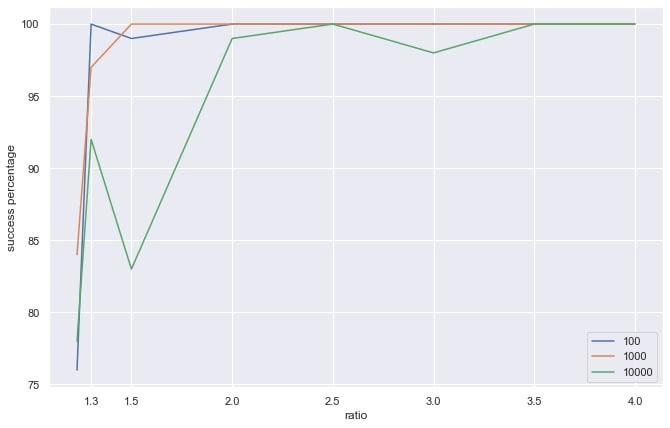
\includegraphics[scale=1.3]{./different_sizes.jpg}
\caption{Recovery rate of subtracted filters. Alice's set of pairs has size of 
10000. Bobs number of pairs correspond to plot lines. Number of hash functions equals 3.}  

\end{figure}


\subsubsection{Recovery of subtraction of two IBLT with the same number of pairs without poisoned keys}

The next table represents Alice-Bob case where they have no intersecting keys. 
Since they both have n pairs, m = 2 * n * ratio.
\\
We can see that the results are similar to the success rate of a simple IBLT:
$f_A - f_B$ is recoverable only iff $f_{A \cup B}$ is recoverable. This happens 
since list entries succeeds only if there is a non empty cell without collision 
on every step of the algorithm. The cell has no collision in $f_{A \cup B}$ iff
the cell has no collision in $f_{A} - f_{B}$. There is a slight possibility that 
count of the cell with collision equals 1 (for example a cell with 2 Alice's pairs
and 1 Bob's pair) and hash of sum coincidentally equals sum of hashes, which is 
so rare that this possibility is negligible. 

\begin{center}
\begin{tabular}{l | l | l | l | l | l} \hline \hline k = 3 \\ \hline
    \hline n & $r = 1.23$ &  $r = 1.3$  &  $r = 1.5$ & $r = 2$ & $r = 3$\\ \hline
    \hline \ 100 & 22.9 & 62.9 & 90.5 & 94.1 & 98.4 \\ \hline 
    1000 & 42.7 & 83.9 & 90 & 95 & 98.8 \\ \hline
    10000 & 78 & 92 & 86 & 100 & 99 \\ \hline
% \end{tabular}
% \\ \\ \\ \\  
% \centering
% \begin{tabular}{l | l | l | l | l | l}
    \hline
    k = 4 \\
    \hline
    \hline n & $r = 1.23$ &  $r = 1.3$  &  $r = 1.5$ & $r = 2$ & $r = 3$\\ \hline
    \hline \ 100 & 0.3 & 19.9 & 83.6 & 91.1 & 98.2 \\ \hline 
    1000 & 0 & 33.8 & 84.8 & 93 & 98.1 \\ \hline
    10000 & 0 & 66 & 78 & 92 & 99 \\ \hline
\end{tabular}
\end{center}

\subsubsection{Recovery of subtraction of two IBLT with the same number of pairs with only poisoned keys}
We can see that the results are close to the results of the recovery of a simple IBLT.
\\
This similarity can be explained by the same logic as 3.2.3: $f_A - f_B$ recovers 
only iff $f_A'$, where all the keys of A set has values equal to 
$value_A - value_B$.
\begin{center}
\begin{tabular}{l | l | l | l | l | l} \hline \hline k = 3 \\ \hline
    \hline n & $r = 1.23$ &  $r = 1.3$  &  $r = 1.4$ & $r = 2$ & $r = 3$\\ \hline
    \hline \ 100 & 10.9 & 31 & 59.2 & 94 & 99.2 \\ \hline 
    1000 & 37.4 & 96.5 & 97.7 & 99.4 & 100 \\ \hline
% \end{tabular}
% \\ \\ \\ \\  
% \centering
% \begin{tabular}{l | l | l | l | l | l}
    \hline
    k = 4 \\
    \hline
    \hline n & $r = 1.23$ &  $r = 1.3$  &  $r = 1.4$ & $r = 2$ & $r = 3$\\ \hline
    \hline \ 100 & 0.3 & 8.7 & 52.7 & 97.3 & 99.3 \\ \hline 
    1000 & 0 & 31.1 & 99.4 & 99.8 & 99.9 \\ \hline
\end{tabular}
\end{center}


\subsubsection{Recovery of subtraction of two IBLT of the same size with different proportions of poisoned keys}
See figure 3. The plot illustrates the recoverability rate for Alice-Bob case
for different number of hash functions, different ratios of poisoned keys and 
ratios equal to 3 and 3.5 (m = 2 * n * ratio). Each line represents number of hash 
functions.

\section{Human genomes and IBLT}
\subsection{VCF}
VCF stands for Variant Call Format. It stores multiple genomes in one file as 
SNP differences between samples and reference genome. 
In the github repository with the IBLT implementation there is a cut copy of a
vcf file, more precisely its few columns containing POS, ID, REF, ALT and 4 SAMPLEs 
from the original vcf file which was found and downloaded in a 1000 Genomes 
Project \textcite{genomes} site.
\begin{figure}[h]
\centering
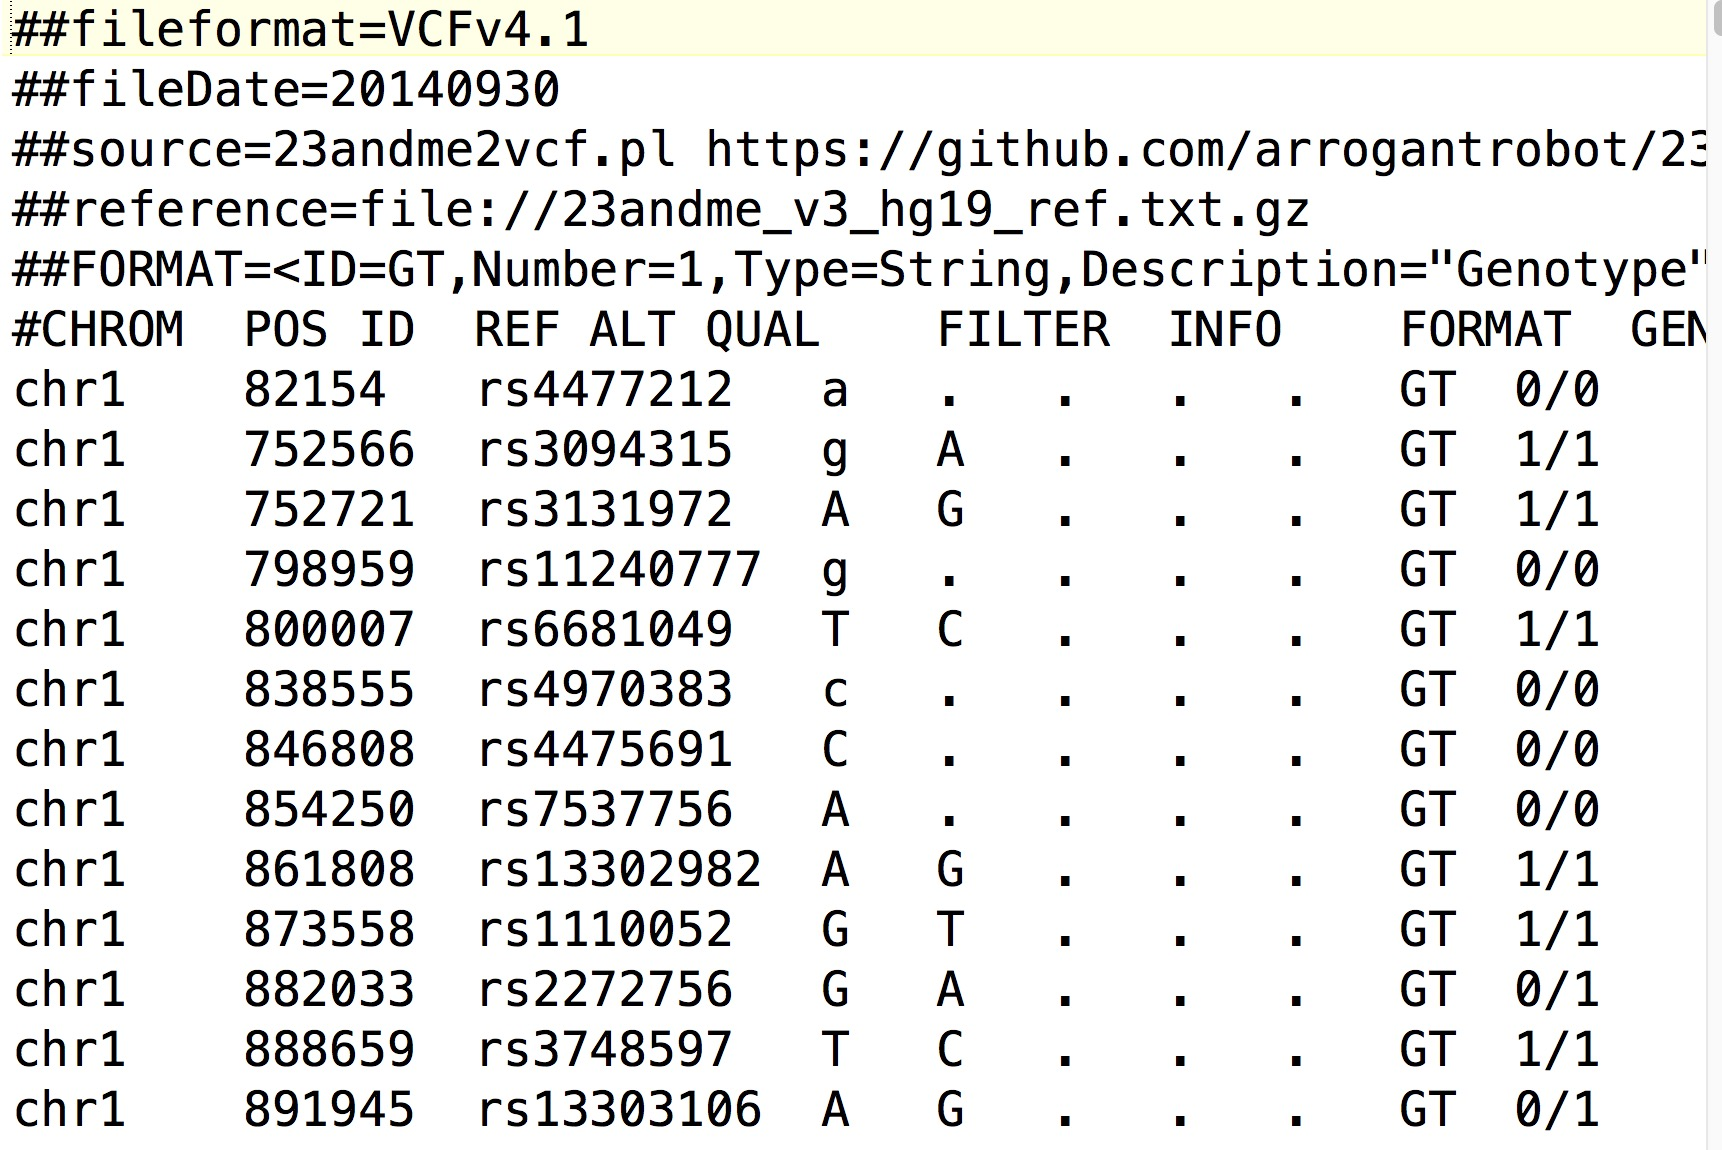
\includegraphics[scale=0.25]{./vcf_format.jpg}
\caption{Example of a VCF file containing first chromosome.
}
\end{figure}
Columns of VCF file interesting to us:
\begin{itemize}
    \item CHROM --- number of the chromosome. In the example it is the 1 out
        of 46 human chromosomes.
    \item POS --- position of the SNP or InDels aligned to the reference genome
        which is reference to all samples in a file.
    \item REF --- value in the position in reference genome.
    \item ALT --- alternative value for the position.
    \item INFO --- in 1000 Genomes VCF these columns are called as human 
        identifiers. Each of 0|0 or 0|1 etc values represent SNP occurrence in 
        each of the chromosome alleles. For example 0|1 would represent that 
        an SNP happened only in the second allele.   
\end{itemize}
\subsubsection{Storing genomes in IBLT}
Storing a VCF in an IBLT is pointless because without reference we can't recover
genome. If we store a reference then using IBLT is also pointless since VCF stores 
it also in O(difference from reference) but with a significantly less constant.
\subsubsection{Comparing genomes in IBLT}
Results of experimenting with comparing two real genomes: \\
62.2\% of successes in 1000 simulations with n = 100, k = 3, ratio = 3. \\
11\% successes in 100 simulations with n = 1000, k = 3, ratio = 3. \\
20\% successes in 10 simulations with n = 10000, k = 3, ratio = 3. \\

Conclusions after simulations:
\begin{itemize}
    \item Success rate is too low.
    \item Ratio is too big (that includes storing multiple arrays and IBLT
        ratio > 1).
    \item Unpacking two genomes takes O(nm) time which is way too long since the
        length of the genomes. 
    \item Results also can be explained by small range of values of key-value 
        pairs --- 0|1, 1|0, 1|1 --- were encoded to 1, 2, 3.
\end{itemize}


\section{Conclusions}
We experimented with an Invertible Bloom Lookup Table and got really good
recoverability rate. IBLT is indeed a very powerful data structure - all its 
variations showed close to 100 percentages with a relatively small ratios. 
Despite all that, experiments with human genome showed negative results for 
this use case: big ratios, small percentage and slow recovery. Thus, without 
new ideas of packing or new ways of applying (we experimented only with packed 
VCF) IBLT is not efficient for storing human genome.
\begin{figure}[h]
\centering
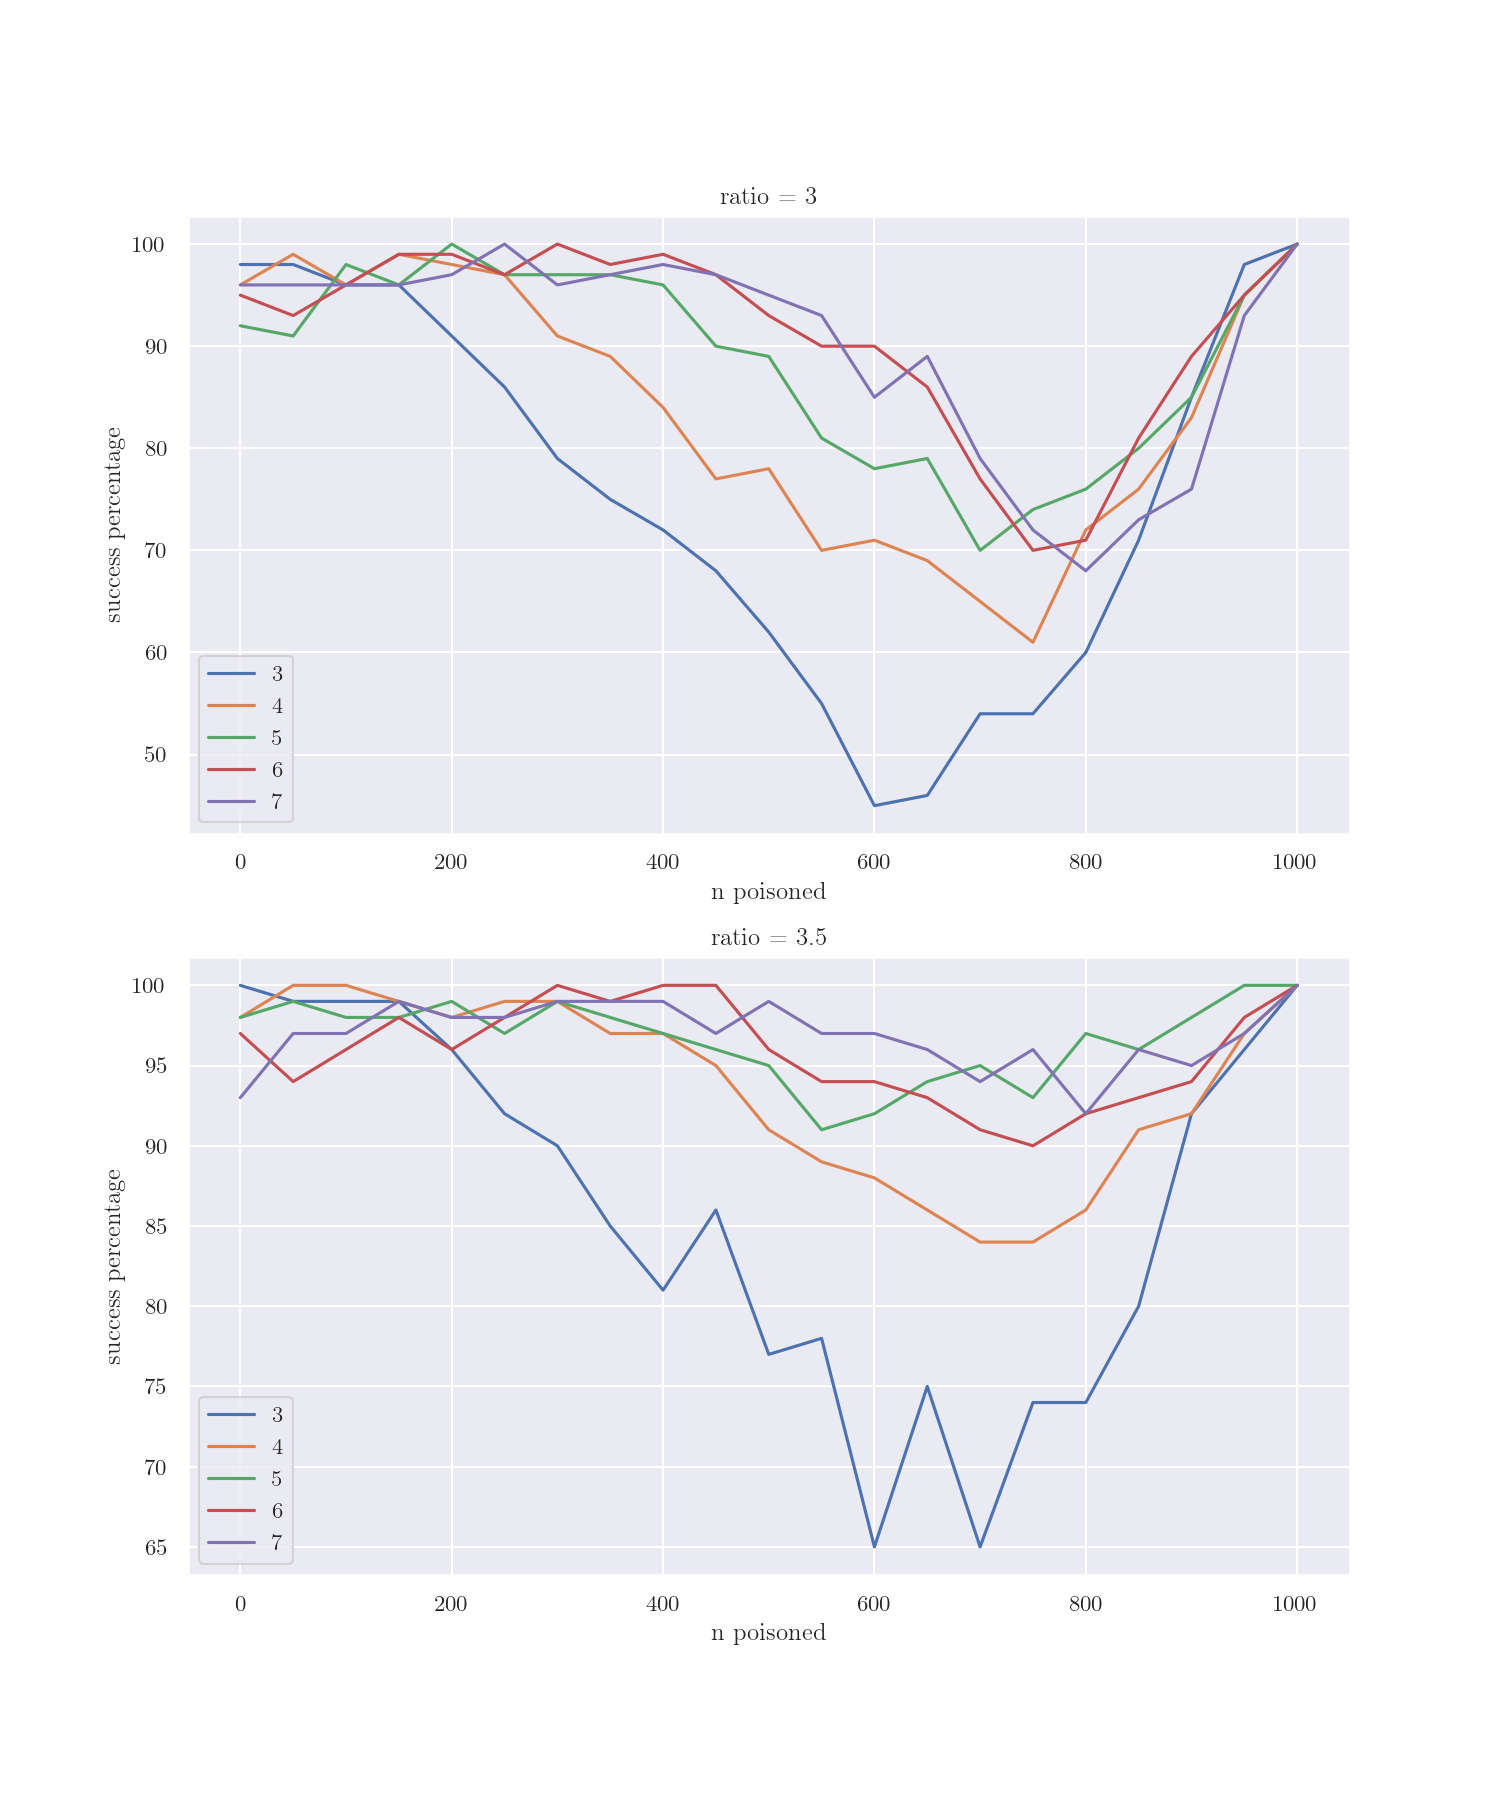
\includegraphics[scale=0.75]{./poisoned50.png}
\caption{Recovery rate of subtraction of two filters (each has 1000 pairs) depending on
number of poisoned keys. Each line represents different number of hash functions.}
\end{figure}


%\begin{enumerate}
%    \item Разработать алгоритм, восстанавливающий числа Бетти пространства по записи активности нейронов гиппокампа грызуна.
%    \item Обратная задача: разработать алгоритм, который, имея пространство известной топологии, генерирует
%        данные, достаточно похожие на запись нейронов гиппокампа грызуна, как если бы тот исследовал это пространство.
%\end{enumerate}
%Для решения этих задач планируется применить инструменты топологического анализа данных вкупе с
%результатами теории нейронных кодов.

%Для решения первой задачи взят за основу алгоритм,
%описанный в статье \textcite{CuIt08}, однако способ генерации активности не учитывает
%поведенческие особенности грызуна и использует упрощенную модель нейронов места, поэтому
%без модификаций этот алгоритм на реальных данных не работает, однако взят за основу.
% в случае компьютерной генерации записи активности нейронов существует алгоритм,
%  модель активности нейронов, использованная там, не учитывает

%Так как 

% Во введении надо кратко описать область, в которой будет ваша работа, потом  
% рассказать о поставленной задаче, далее о том, что вы будете делать.В конце  
% введения обычно принято писать обзор структуры содержательной части, чтобы   
% можно было сориентироваться в происходящем, не начиная читать содержательную 
% часть.

% \textcite{GGO} says
% Note also that very recently several constructions of~\cite{Elkik73} were clarified and simplified by Gabber and Ramero in~\cite[Chapter~5]{GabRam}. Some other source with url~\cite{GGO}

%\section{Методы}
%\subsection{Данные}
%Наши данные --- записи нейронной активности нескольких мышей, которые
%блуждают по круглым аренам с разной топологической структорой --- с 1, 2 или 3 пустотами.

%\subsection{Декодирование топологии}

%\subsection{Генерация нейронной активности}

%\section{Результаты}

%\section{Обсуждение}

% С этого момента глобальная нумерация идет буквами. Этот раздел я добавил лишь для демонстрации возможностей LaTeX, его можно и нужно удалить и он не нужен для курсового проекта непосредственно.
%\appendix

%\section{Математическая терминология}
% число, сохраняющееся после непрерывных преобразований пространства, 
%Число Бетти $\beta_i$ топологического пространства --- количество $i$-мерных
%пустот в нем. При этом нулевое число Бетти --- число компонент связности топологического пространства.
%Для графа $\beta_i$ --- количество независимых циклов в графе, например, у дерева
%$\beta_i = 0$. А, например, у геометрического объекта --- окружности $S_1$ --- $\beta = 1$.

\printbibliography

% Проведем небольшой обзор возможностей \LaTeX. Далее идет обзорный кусок, который надо будет вырезать. Он приведен лишь для демонстрации возможностей \LaTeX.
%
% \section{Нумеруемый заголовок}
% Текст раздела
% \subsection{Нумеруемый подзаголовок}
% Текст подраздела
% \subsubsection{Нумеруемый подподзаголовок}
% Текст подподраздела
%
% \section*{Не нумеруемый заголовок}
% Текст раздела
% \subsection*{Не нумеруемый подзаголовок}
% Текст подраздела
% \subsubsection*{Не нумеруемый подподзаголовок}
% Текст подподраздела
%
%
% \paragraph{Заголовок абзаца} Текст абзаца
% Формулы в тексте набирают так $x = e^{\pi i}\sqrt{\text{формула}}$. Выключенные не нумерованные формулы набираются либо так:
% \[
% x = e^{\pi i}\sqrt{\text{формула}}
% \]
% Либо так
% $$
% x = e^{\pi i}\sqrt{\text{формула}}
% $$
% Первый способ предпочтительнее при подаче статей в журналы AMS, потому рекомендую привыкать к нему.
%
% Выключенные нумерованные формулы:
% \begin{equation}
% \label{Equation1}
% % \label{имя-метки} эта команда ставит метку, на которую потом можно сослаться с помощью \ref{имя-метки}. Метки можно ставить на все объекты, у которых есть автоматические счетчики (номера разделов, подразделов, теорем, лемм, формул и т.д.
% x = e^{\pi i}\sqrt{\text{формула}}
% \end{equation}
% Или не нумерованная версия
% \begin{equation*}
% x = e^{\pi i}\sqrt{\text{формула}}
% \end{equation*}
%
% Уравнение \ref{Equation1} радостно занумеровано.
%
% Лесенка для длинных формул
% \begin{multline}
% x = e^{\pi i}\sqrt{\text{очень очень очень длинная формула}}=\\
% \tr A - \sin(\text{еще одна очень очень длинная формула})=\\
% \cos z \Im \varphi(\text{и последняя длинная при длинная формула})
% \end{multline}
%
% Многострочная формула с центровкой
% \begin{gather}
% x = e^{\pi i}\sqrt{\text{очень очень очень длинная формула}}=\\
% \tr A - \sin(\text{еще одна очень очень длинная формула})=\\
% \cos z \Im \varphi(\text{и последняя длинная при длинная формула})
% \end{gather}
%
% Многострочная формула с ручным выравниванием. Выравнивание идет по знаку $\&$, который на печать не выводится.
% \begin{align}
% x = &e^{\pi i}\sqrt{\text{очень очень очень длинная формула}}=\\
% &\tr A - \sin(\text{еще одна очень очень длинная формула})=\\
% &\cos z \Im \varphi(\text{и последняя длинная при длинная формула})
% \end{align}
%
% \begin{theorem}
% Текст теоремы
% \end{theorem}
% \begin{proof}
% В специальном окружении оформляется доказательство.
% \end{proof}
%
% \begin{theorem}[Имя теоремы]
% Текст теоремы
% \end{theorem}
% \begin{proof}[Доказательство нашей теоремы]
% В специальном окружении оформляется доказательство.
% \end{proof}
%
% \begin{definition}
% Текст определения
% \end{definition}
%
% \begin{remark}
% Текст замечания
% \end{remark}
%
% \paragraph{Перечни:} Нумерованные
% \begin{enumerate}
% \item Первый
% \item Второй
% \begin{enumerate}
% \item Вложенный первый
% \item Вложенный второй
% \end{enumerate}
% \end{enumerate}
%
% Не нумерованные
%
% \begin{itemize}
% \item Первый
% \item Второй
% \begin{itemize}
% \item Вложенный первый
% \item Вложенный второй
% \end{itemize}
% \end{itemize}
\end{document}
